\begin{pastexam}[label={px:ntust-106-ice-03}]{臺科大資工所 106 學年度 第 3 題}
（問答）

Stack/Queue (10\%)

Consider an infix expression as follows.

\hspace*{4em}((d-e)/((a+b)*(c-d)))/f
\begin{enumerate}[label=(\alph*)]
\item What is the corresponding prefix expression? (5\%)
\item What is the corresponding postfix expression? (5\%)
\end{enumerate}
\end{pastexam}

\begin{pastsoln}
答案：(a) ${/}\,{/}\,{-}\,d\,e\,{*}\,{+}\,a\,b\,{-}\,c\,d\,f$；(b) $d\,e\,{-}\,a\,b\,{+}\,c\,d\,{-}\,{*}\,{/}\,f\,{/}$。

先畫運算式樹（資結書第~7.7~節）：最外層是「$(\ldots)/f$」，根是右邊那個 $/$；它的左子樹是
$(d-e)/((a+b)*(c-d))$，再往下拆。
\begin{center}
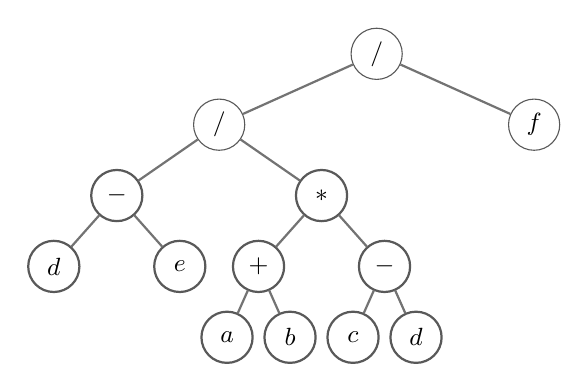
\begin{tikzpicture}[level distance=9mm,
  every node/.style={circle,draw=black!65,minimum size=6.5mm,inner sep=0pt,font=\small},
  edge from parent/.style={draw=black!55,thick},
  level 1/.style={sibling distance=40mm},
  level 2/.style={sibling distance=26mm},
  level 3/.style={sibling distance=16mm},
  level 4/.style={sibling distance=8mm}]
\node {$/$}
  child {node {$/$}
    child {node {$-$}
      child {node {$d$}}
      child {node {$e$}}}
    child {node {$*$}
      child {node {$+$}
        child {node {$a$}}
        child {node {$b$}}}
      child {node {$-$}
        child {node {$c$}}
        child {node {$d$}}}}}
  child {node {$f$}};
\end{tikzpicture}
\end{center}
前序走訪就是前序式，後序走訪就是後序式（資結書第~7.3~節）。 運算元的順序不變，都是
$d, e, a, b, c, d, f$，只有運算子的位置不同。

\textbf{(a) 前序式}（根、左、右）：根 $/$；左子樹的前序是 $/$、${-}\,d\,e$、${*}\,{+}\,a\,b\,{-}\,c\,d$；最後右子樹 $f$：
\[
{/}\ {/}\ {-}\ d\ e\ {*}\ {+}\ a\ b\ {-}\ c\ d\ f.
\]

\textbf{(b) 後序式}（左、右、根）。 也可以用資結書虛擬碼~6.8 的堆疊轉換，左括號推入、右括號彈出到
左括號為止，同級的 $/$ 遇到 $/$ 要先彈出（由左往右結合）：
\begin{center}
\small
\begin{tabular}{cll}
\toprule
讀到 & 堆疊（左邊是底） & 輸出 \\
\midrule
$(\ (\ d$ & $(\ ($ & $d$ \\
${-}\ e$ & $(\ (\ {-}$ & $d\,e$ \\
$)$ & $($ & $d\,e\,{-}$ \\
$/$ & $(\ {/}$ & $d\,e\,{-}$ \\
$(\ (\ a\ {+}\ b$ & $(\ {/}\ (\ (\ {+}$ & $d\,e\,{-}\,a\,b$ \\
$)$ & $(\ {/}\ ($ & $d\,e\,{-}\,a\,b\,{+}$ \\
${*}\ (\ c\ {-}\ d$ & $(\ {/}\ (\ {*}\ (\ {-}$ & $d\,e\,{-}\,a\,b\,{+}\,c\,d$ \\
$)$ & $(\ {/}\ (\ {*}$ & $d\,e\,{-}\,a\,b\,{+}\,c\,d\,{-}$ \\
$)$ & $(\ {/}$ & $d\,e\,{-}\,a\,b\,{+}\,c\,d\,{-}\,{*}$ \\
$)$ & （空） & $d\,e\,{-}\,a\,b\,{+}\,c\,d\,{-}\,{*}\,{/}$ \\
${/}\ f$ & $/$ & $d\,e\,{-}\,a\,b\,{+}\,c\,d\,{-}\,{*}\,{/}\,f$ \\
結束 & （空） & $d\,e\,{-}\,a\,b\,{+}\,c\,d\,{-}\,{*}\,{/}\,f\,{/}$ \\
\bottomrule
\end{tabular}
\end{center}
（連續的運算元、左括號和運算子合成一列寫。）結果和樹的後序走訪相同：
\[
d\ e\ {-}\ a\ b\ {+}\ c\ d\ {-}\ {*}\ {/}\ f\ {/}.
\]
可以用後序求值驗算：$d\,e\,{-}$ 得 $d-e$；$a\,b\,{+}$ 得 $a+b$；$c\,d\,{-}$ 得 $c-d$；$*$ 得 $(a+b)*(c-d)$；
$/$ 得 $(d-e)/((a+b)*(c-d))$；$f\,{/}$ 得整個式子。
\end{pastsoln}
